% !TEX root = ../arbeit.tex
\chapter{Related Work}\label{chapter:relatedWork}
Presenting content on a large surface is typically done by an ordinary projector. Over the last decade various ideas have been developed to extend the capabilities and integrate projectors into more sophisticated systems. Potential systems range from simple keystone correction over mobile projection to fully environment sensing systems which are capable of augmenting recognised objects with an overlay. The \ac{HCI} community has done research on various types of user interaction, especially on augmented environment interactive projection interfaces. Following, a brief overview is given over several wearable or handheld  as well as mounted systems which are correlated to this thesis. Additionally frameworks enabling rapid prototyping for mobile projector interaction techniques or for development of interactive projection based displays are examined. 

\section{Wearable and Handheld Systems}
The research of wearable and handheld \acfp{PROCAMS} focus in particular on mobile interaction concepts and the development of small units providing information access everywhere we go. 

Such PROCAMS could be attached to different positions. For example shoulder, hip, back of the hand or the head. \textcite{McFarlane:2009jz} analysed several of theses possibilities to minimise situational impairments since it can affect primary task like using the phone while driving. They developed \textit{Interactive Dirt}, a simple \ac{PROCAMS} from stock hardware under the aspect to minimise negative effects to situational awareness and enable easy interaction.  
The systems performance is evaluated in a field study with military background. In a semi-structured usability trial the left shoulder is discovered as the positions with best characteristic for supporting mobile teamwork. Challenges discovered in this trails are the lack of uniform surfaces in non urban environments as well as the brighter ambient lighting.~\citeauthor{McFarlane:2009jz} named instant access to a large display while hands free one as one of the biggest benefits of a \ac{PROCAMS}.  

Focusing on novel freehand gestural interaction~\textcite{Pranavv:2009bo} develop a interactive system containing a projector, a camera and coloured markers on the finger to track gestures (see \autoref{img:sixSetup}). In addition interaction with different augmented physical objects (see \autoref{img:sixAugmented}) is possible. Popular interactive multitouch based gestures as pinch to zoom are developed. Tending a wide distribution of the system~\citeauthor{Pranavv:2009bo} distributed \textit{SixthSense} as an open source project~\cite{Pranavv:2013ng}. Furthermore, they planed to improve the prototype by markerless tracking, distortion free projection as well as a smaller form factor. The proposed system shows already that complex interactions are possible with average hardware however markers were necessary. Moreover distortion free rendering is not yet realised since it is very complex and computational expensive with the proposed hardware. 

\begin{figure}
        \centering
        \begin{subfigure}[b]{0.3\textwidth}
               \def\svgwidth{\textwidth}
               {\fontfamily{phv}\selectfont \import{images/relatedwork/}{sithsense.pdf_tex}}
               % 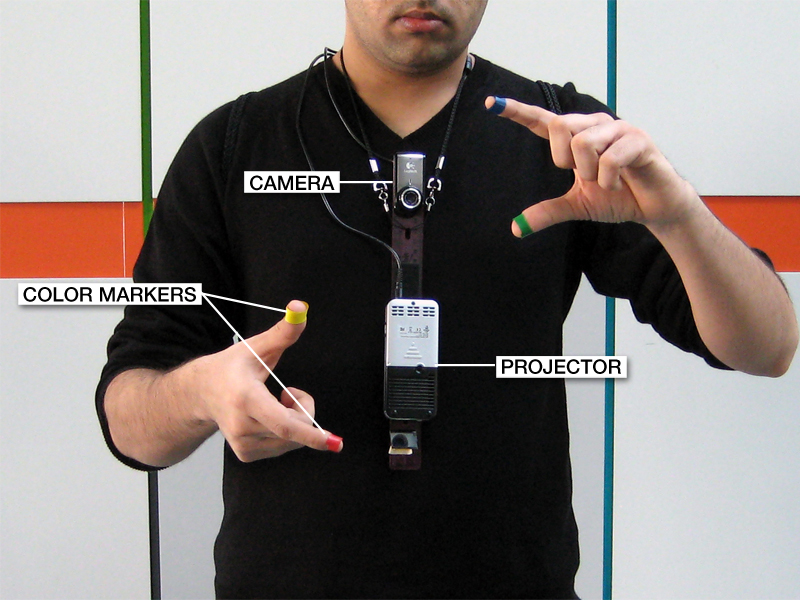
\includegraphics[width=\textwidth]{images/relatedwork/sixthsense01.jpg}
                \caption{SixthSense hardware\newline}
                \label{img:sixSetup}
        \end{subfigure}
         \quad %add desired spacing between images, e. g. ~, \quad, \qquad etc.
          %(or a blank line to force the subfigure onto a new line)
        \begin{subfigure}[b]{0.3\textwidth}
                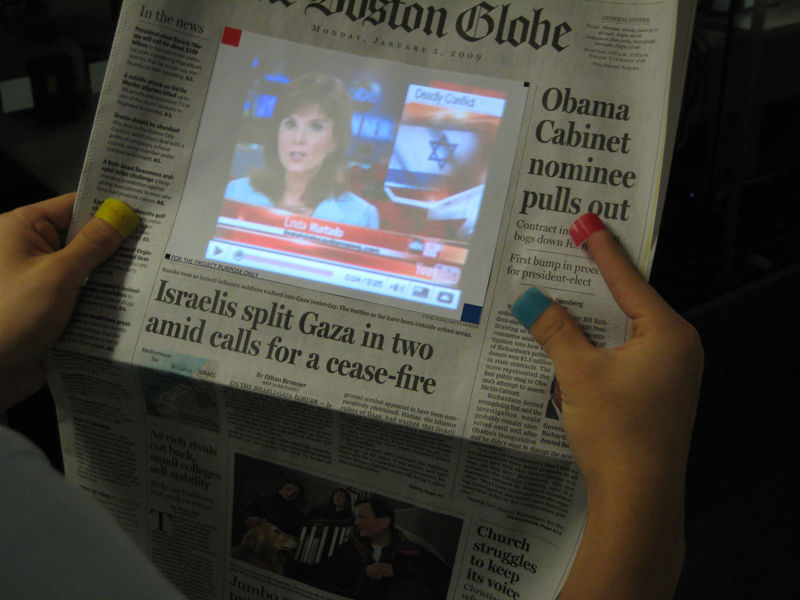
\includegraphics[width=\textwidth]{images/relatedwork/sixthsense02.jpg}
                \caption{Augmenting physical objects with SixthSense }
                \label{img:sixAugmented}
        \end{subfigure}
         \quad%add desired spacing between images, e. g. ~, \quad, \qquad etc.
          %(or a blank line to force the subfigure onto a new line)
        \begin{subfigure}[b]{0.3\textwidth}
        \setlength\fboxsep{0pt}
        \fbox{   
              \def\svgwidth{\textwidth}            
{\fontfamily{phv}\selectfont \import{images/relatedwork/}{brain.pdf_tex}}
               }%fbox
	      %\input{images/relatedwork/brain.pdf_tex}
                %\includegraphics[width=\textwidth]{images/interview/bainyhand.jpg}
                \caption{Brainy Hand\newline}
                \label{img:bainyhand}
        \end{subfigure}
        \caption{Mobile Systems}\label{fig:animals}
\end{figure}

Another system similar to \textit{SixthSense} which also allows interaction with physical objects is the \ac{PROCAMS} by~\textcite{Mobileprojectorcam:tw}. Here the \ac{PROCAMS} is not wearable but handheld. It is capable of augmenting physical objects with meta information. A flashlight metaphor as interaction concept which present stored metadata next to the illuminated object is used. Recognition is done via computer vision using  motion and feature tracking. Compared to the \textit{SixthSense} prototype features are matched against a database which makes separate markers redundant.

Presented and developed systems are often to bulky for everyday usage.~\textcite{Tamaki:2009hr} focus on this issue and propose \textit{Brainy Hand}, a wearable hand gesture interaction device. They show that it is entirely possible to construct very small PROCAMS but with a tradeoff of flexibility in feedback and interaction.~\citeauthor{Tamaki:2009hr}describe two different devices. A simple one containing only a small camera to estimate 3D hand gestures as input and a laser to indicate the field of view. The second version additionally includes a projector to display visual feedback. The concept of \textit{Brainy Hand} is illustrated in~\autoref{img:bainyhand}. A novel 3D hand gesture estimation technique which does not require any marker was used to detect up to five gestures including point, motion and sign gestures. With an implemented music player application the feasibility of the prototype has been shown.

\textcite{Molyneaux:2012wo} present a novel environment aware projector to enable new interaction method. To enable spatial and geometrical awareness they pursue two different approaches. On the one hand, they develop a \ac{PROCAMS} which is tracked by a tracking system deployed in the environment. This enables environmental aware distortion free projection as well as  novel freehand user interactions du to the tracking of the user. One disadvantage of this approach is the need of a deployed tracking system. The second \ac{PROCAMS} is equipped with Microsoft Kinect which enables to determine the pose in space via simultaneous localisation and mapping (SLAM) technique. This allow spatial aware projection and re-projection without any infrastructure. 

\textit{Interactive Phone Call} by~\textcite{Winkler:2011kk} provides in call collaboration while making a telephone call. Therefore they proposed to attach a pico projector to a mobile phone to project content to a flat surface. This allows the user to interact and share content with one hand while holding the phone in the other.~\citeauthor{Winkler:2011kk} use a desktop metaphor with a private and a shared area and additional extended permissions for file sharing.


\textit{OmniTouch} by~\textcite{Harrison:2011bn} is a shoulder-worn portable \ac{PROCAMS}. Multitouch interaction on planar surfaces is provided by a depth sensing camera.~\citeauthor{Harrison:2011bn} propose that with \textit{OmniTouch} they can provide phone like interfaces in the palm of the hand. Projecting content as well as multitouch interaction works without calibration nor instrumentation of the environment. Hence geometrical awareness is limited to the depth sensing camera data. Spatial awareness is not provided.

\textcite{Winkler:2014wp} present the \textit{Ambient Mobile Pervasive Display} concept. The hardware composition of the prototype is very similar to \textit{OmniTouch}~\cite{Harrison:2011bn}.~\citeauthor{Winkler:2014wp} refine this idea. A constantly projection in front of the use to project public information as well as a projection in the palm of the hand for private information on demand is provided. In contrast to \textit{OmniTouch}, the build prototype has geometrical and spatial awareness due to the used sensors. 


There are several HCI research groups which focus on mobile interactive projector systems. Still, there are several issues and challenges to overcome. Systems offering advanced input methods require advanced algorithm and powerful hardware which reduces battery live or even mobility. For mobility purpose pico-projectors are used, but they require room lighting to be significantly dimmed and make outdoor use fairly impossible. Others systems even need an instrumentation of the environment. 
But there are first approaches to solve some of these problems by more sophisticated computer-vision based techniques or by applying more sensors to the build prototypes. 
A lot new questions arise form the proposed systems. For example, which is the most intuitive and comfortable way to interact with such portable systems. Especially in public. Or, more technically questions, is it possible to project undistorted 3D objects on non-planar surfaces. It might be reasonably assumed that over the coming years, as the various underlying technologies get improved, mobile \ac{PROCAMS} could become widely distributed.


\section{Mounted Systems}
Mounted PROCAMS are systems which are basically constructed in laboratories to evaluate new interaction concepts in a domestic environment or how the physical and digital world could blend together for example by augmenting physical objets with meta information. 

More than 20 years ago \citeauthor{Wellner:1991ws} present the \textit{DigitalDesk Calculator}~\cite{Wellner:1991ws}. This is one of the first approaches to merge the physical world with the digital. He propose a fixed \ac{PROCAMS} to enable touch interaction on a desk as well as concepts to transfer paper documents to electronic ones and vice versa. Touch point detection is done by simple image processing. The camera is mounted on top of the desk which makes tap detection difficult. Hence~\citeauthor{Wellner:1991ws} use a microphone to detect taps. 

\textcite{Pinhanez:2001vn} propose \textit{Everywhere Display}, a novel \ac{PROCAMS} which can project to several predefined surfaces. A rotating mirror placed over the projector enables a movable projection cone. A also movable camera is used for interaction input. A schematic setup and the prototype are illustrated in~\autoref{img:everywherdisplay}.~\citeauthor{Pinhanez:2001vn} discus several problems and suitable solutions in his work. User interfaces can be projected distortion free, but  each surface has to be calibrated by hand. New challenges accompanied by the steerable projection as the loss of focus, the loss of resolution involved by projection distance or more complex interaction analysis are identified. Oblique projection of content is for example computed by standard hardware by adapting 3D graphics rendering concepts. 

\textcite{Fails:2002du} focused on a low cost solution for ubiquitous interaction. They proposed \textit{Light Widgets} which makes use of inexpensive cameras to detect skin coloured objects in certain areas of the image to trigger events. Interfaces are manually calibrated in the still image of the camera. Since projectors are expensive \citeauthor{Fails:2002du} provide feedback via a XWeb interaction platform which distribute it to any connected output modality like TVs, the traditional desktop or speech. This work shows that even with cheap hardware ubiquitous indoor interaction is feasible however a instrumenting the environment and manual calibration is mandatory.

\begin{figure}
        \centering
         \subcaptionbox{Everywhere display projector setup\label{img:everywherdisplay01}}
[.52\textwidth]{\def\svgwidth{.60\textwidth} 
{\fontfamily{phv}\selectfont \import{images/relatedwork/}{ep01.pdf_tex}}}
\hfill
         \subcaptionbox{Everywhere display projector setup}
	[.25\linewidth]{\def\svgwidth{0.25\textwidth} {\fontfamily{phv}\selectfont \import{images/relatedwork/}{ep02.pdf_tex}}}
        \caption{Everywhere display projector \cite{Pinhanez:2001vn}}
        \label{img:everywherdisplay}
\end{figure}


Andy Wilson is a principal researcher at Microsoft Research focused on depth sensing interaction techniques \cite{Wilson:2010de,Wilson:2010bv} as well as wearable \cite{Harrison:2011bn} and mounted PROCAMS. In \citeyear{Wilson:2012fb} \citeauthor{Wilson:2012fb} proposed the \textit{Beamatron}, the first movable projector with depth camera. The depth sensing camera allows geometrically aware projection. They managed to project information on moving objects in the physical world. Moreover, the user is tracked and can grab a digital item, carry it through space and place it somewhere else as desired. Alternatively the user can grab items via audio command while pointing at them. Here interaction is only limited by the view frustum of the depth sensing camera. In addition \citeauthor{Wilson:2012fb} develop a novel menu in space where the user select items depending on the height of the hand above the table.

\textcite{Linder:2010cu} introduce \textit{LuminAR}, a projected augmented reality interface, which dynamically augments objects and surfaces with digital information. \textit{LuminAR} consists of a pico-projector,  a camera, and wireless computer in a compact form factor suitable to be embedded in everyday objects like a desk lamp (see~\autoref{img:luminar}). The idea based on \cite{Underkoffler:1999iv} but is enhanced in several ways. \citeauthor{Linder:2010cu} add robotic movement to the desk lamp to  enable dynamic motion capabilities. Hence interaction space and augmentation experiences are increased. 
With the objective of augmented reality becoming mainstream \textcite{Weissmann:2013uj} publish \textit{LENS} a Javascript framework for easy application development for the \textit{LuminAR} platform. This framework provides a API for multitouch, marker and contour tracking, connectivity and decouples complexity from the application. 



In contrast to the movable \textit{LuminAR} system, \textcite{Hardy:2012jo} propose a fixed hardware setup. He presents a software toolkit designed to enable rapid development of multitouch enabled interactive projection-based displays. His framework based on the .NET framework and only requires a ordinary projector, a Microsoft Kinect and a Windows workstation. All challenges involved into interactive projections are decoupled from the application which is a simple HTML5 web page. Interaction like multitouch are injected into these websites. As shown in \autoref{img:hardy} it is possible to simultaneously project displays distortion free to diverse aligned flat surfaces. Still a manual calibration task is necessary. The toolkit capabilities and performance are evaluated. Interestingly touch accuracy, excluding extreme cases, mainly depends on the distance to the surface not on the angle.  

In a long term study over one year \textcite{Hardy:2012ej} evaluated the impact of a \ac{PROCAMS} on general office productivity. The \ac{PROCAMS} depicted in~\autoref{img:hardyLT} is deployed above his desk and offers stylus input. Positively mentioned are the physical integration of the system, the management of notes and collaborative working on ideas as well as the logical differentiation between the projection and the real displays. On the other hand \citeauthor{Hardy:2012ej} criticise the low resolution of only 20 dpi and the bright light of the projection which makes it unpleasant to read or focus on the projection for a longer period of time. A lack of multiuser support and the single input are other limitations. Occlusions are not necessarily a problem as he is sitting most of the time at the desk which does not lead to significant occlusions.
\citeauthor{Hardy:2012ej} outlines that the proposed interactive table is a transitional vision and no replacement for a personal computer. 

\begin{figure}
        \centering
        \begin{subfigure}[b]{0.3\textwidth}
                \includegraphics[width=\textwidth]{images/relatedwork/luminar.jpg}
                \caption{\textit{LuminAR} prototype\newline}
                \label{img:luminar}
        \end{subfigure}
        \quad%add desired spacing between images, e. g. ~, \quad, \qquad etc.
        \begin{subfigure}[b]{0.3\textwidth}
               %\def\svgwidth{\textwidth}
               %\import{images/relatedwork/}{brain.pdf_tex}
                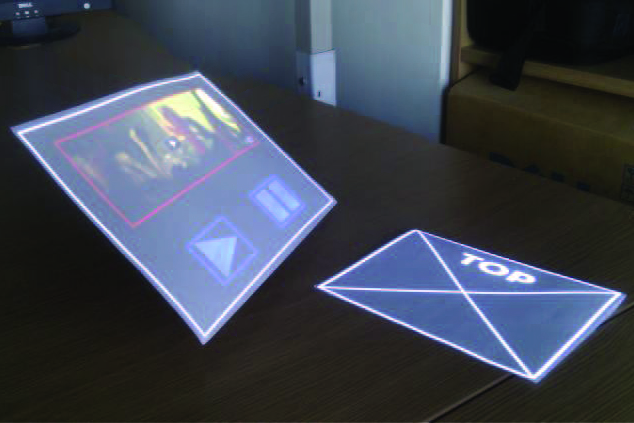
\includegraphics[width=\textwidth]{images/relatedwork/hardy.jpg}
                \caption{Undistorted projections to flat surface}
                \label{img:hardy}
        \end{subfigure}
        \quad %add desired spacing between images, e. g. ~, \quad, \qquad etc.
          %(or a blank line to force the subfigure onto a new line)
          %(or a blank line to force the subfigure onto a new line)
        \begin{subfigure}[b]{0.3\textwidth}      
               %\def\svgwidth{\textwidth}
               %\import{images/relatedwork/}{brain.pdf_tex}
                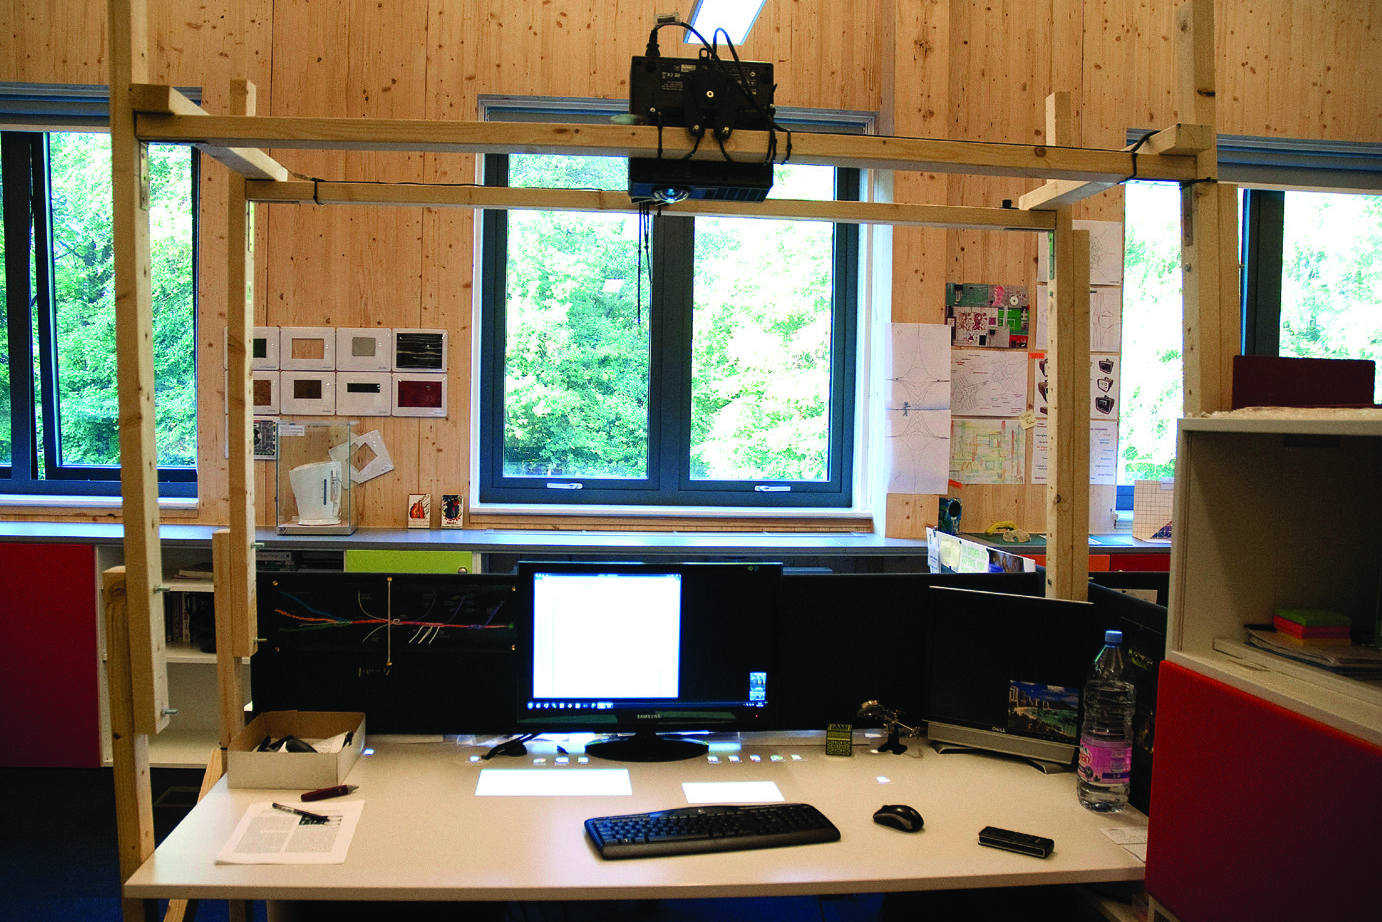
\includegraphics[width=\textwidth]{images/relatedwork/hardy02.jpg}
                \caption{Long term study environment}
                \label{img:hardyLT}
        \end{subfigure}
        \caption{Mobile Systems}\label{fig:animals}
\end{figure}

Achieving ubiquitous computing \citeauthor{Xiao:2013dp} propose the \textit{WorldKit} system \cite{Xiao:2013dp}. Using a paired depth camera and projector, user interfaces can interactively placed on nearly any surface by simply rubbing the surface with the flat hand.
Compared to \textit{LuminAR} and the toolkit by Hardy none manual calibration of surfaces or setup tasks are necessary. Furthermore, the WorldKit systems implemented a \emph{interactor} library offering a variety of interaction types like contact, contact area, number of contacts or colour and brightness. The system encapsulates these capabilities to enable easy and rapid development of novel interfaces. \citeauthor{Xiao:2013dp} expect that this abstractions make the new ubiquitous computing accessible for more developers. 


Overall, there is an increase in proposed systems and toolkits over the last decade. Starting from \citeauthor{Wellner:1993vh} idea 1991 researchers develop systems to achieve ubiquitous computing. Beginning with easy interaction realised with simple cameras and manual configuration tasks, the release of the Microsoft Kinect provides a inexpensive solution for novel interaction concepts. Systems and toolkits get enhanced from static to movable \ac{PROCAMS} offering more accurate touch input and simple application development by providing simplified APIs. Nowadays \ac{PROCAMS} enable ubiquitous, on demand creation of interactive interfaces without manual calibration tasks. 
Issues and challenges know form portable systems like power management or computational power are not crucial but there are still  hardware limitations like interaction accuracy or projection resolution. Furthermore all presented systems are tied to laboratory. Non of them where actually used to conduct user studies in a domestic environment. 

\section{Commercially Available Products}

To give a complete overview of the current PROCAMS evolution, commercially available products for educationally use, entertainment or advertisement are discussed in the following.

 \begin{figure}[htbp]
        \centering
        \begin{subfigure}[b]{0.48\textwidth}
                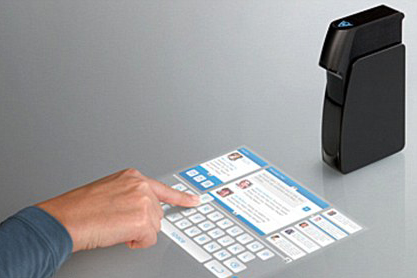
\includegraphics[width=\textwidth]{images/relatedwork/lbo.jpg}
                \caption{\emph{Light Touch} by Light Blue Optics\footnotemark}
                \label{img:lbo}
        \end{subfigure}
        \hfill
        \begin{subfigure}[b]{0.48\textwidth}      
                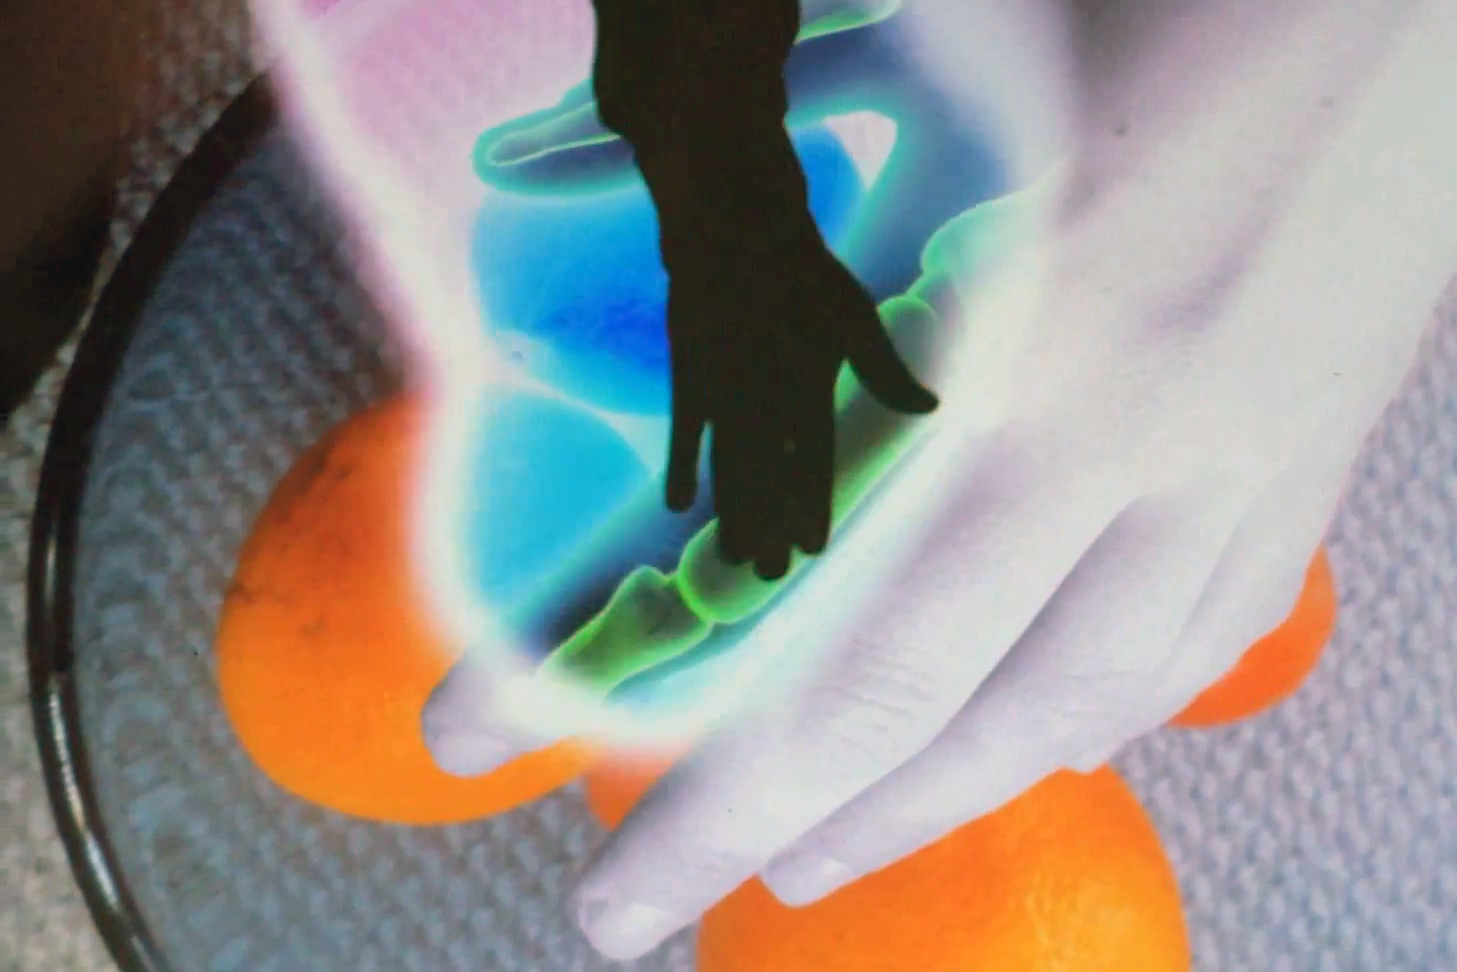
\includegraphics[width=\textwidth]{images/relatedwork/omi.jpg}
                \caption{omiVista by OM Interactive}
                \label{img:omi}
        \end{subfigure}
        \caption{Commercial products}\label{fig:animals}
\end{figure}
\footnotetext{\url{http://www.engadget.com/products/light-blue-optics/light-touch}}

\pagebreak
The startup Light Blue Optics~\cite{Blue:2014ab} launches \textit{Light Touch}\cite{Anonymous:NA7eH3SN} at the Consumer Electronics Show in 2010. \textit{Light Touch} is a standalone \ac{PROCAMS} with novel laser projection technology which turns flat surface into a touch screen. Due to the laser projection the image is always in focus. The device supports multitouch via camera tracking. Simple applications like photo manager, movie player, or messaging service are presented. Sadly the projection area of the device is very limited and seems like a tablet. Interaction is heavily based on concepts known from current smart phones. However, the small stand-alone character of the final product which is shown in~\autoref{img:lbo} is very appealing. 

OM Interactive motivated their products for the education and health sector. They sell and rent different interactive projection systems for different setup situations like wall, floor or ceiling projection. All interactive systems are powered by the \textit{EyeClick} engine which respond to gestures or movement tracked by a infrared camera system. Gesture information are forwarded to a computer which adjusts the content. Because the gesture recognition appears to be not very accurate user interface elements are very large or the interaction concept does not require direct selection of objects.
A sample template showing the \text{omiVista}~\cite{Anonymous:QJL7w_S-} is illustrated in~\autoref{img:omi}. Other companies offering similar products as OM Interactive are GestureTek or Reactrix Systems. Later are focused in particular on out-of-home advertising, retail, and entertainment. The used technologies and scope of operation are basically the same described above.